\section{Omfang af belægning}
På ortopædkirurgisk afdeling på Aalborg Universitetshospital ses en varierende belægningsgrad fra måned til måned. Belægningsgraden er antallet af disponible senge i brug. På \figref{maxminbelaeg} ses den varierende belægning fra år $2014$ til $2015$ på ortopædkirurgisk afdeling. \cite{SDS2015}


\begin{figure}[H]
	\flushleft 
	\centering
	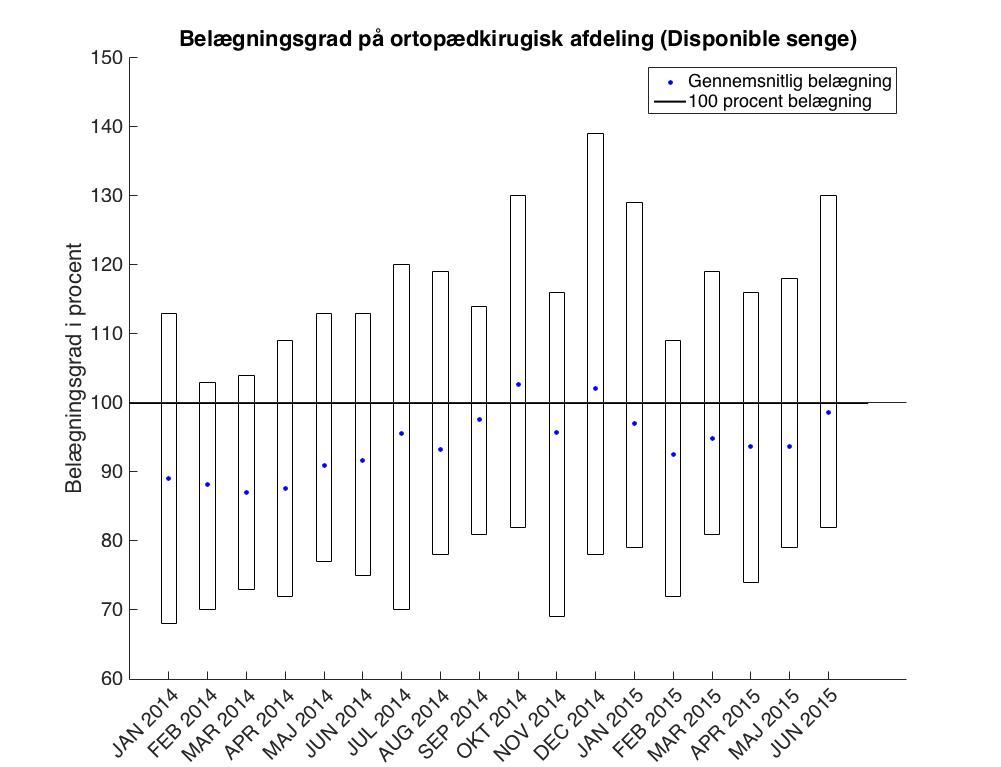
\includegraphics[scale=.45]{figures/maxminoverbelaeg.png}
	\label{maxminbelaeg}
	\flushleft
	\caption{\textit{Figuren illustrerer belægningsgraden over 18 måneder fra år $2014$ til $2015$ på ortopædkirurgisk afdeling på Aalborg Universitetshospital. Søjlerne viser belægning ift. $100\%$ belægning, dertil ses den gennemsnitlige belægning for hver måned som et punkt. \cite{SDS2015}}}
\end{figure}


Det fremgår af \figref{maxminbelaeg}, at ortopædkirurgisk afdeling oplever en belægning hhv. over og under én ønskede belægning på $100 \%$. I december måned år $2014$ ses en maksimal belægning på $1XX \%$ og en minimums belægning på $xx \%$. Dette indikerer, at ortopædkirurgisk afdeling oplever belægning over $100 \%$ i kortvarige perioder. Da \figref{maxminbelaeg} ikke viser belægningsperioden er det uvist om, hvorvidt belægningen over $100 \%$ opleves i timer eller flere dage. Der skal herudover tages forbehold for, at \figref{maxminbelaeg} både indeholder elektive samt akutte indlagte patienter, og derfor er uvist om, hvorvidt det er akutte patienter, der resulterer i en belægningsgrad på over $100 \%$. Der ses ligeledes en gennemsnitlig belægning pr. måned på \figref{maxminbelaeg}. Denne ses hyppigst under $100 \%$ belægning, hvortil der kun ses oktober samt december i år $2014$ med en gennemsnitlig belægning på over $100 \%$ belægning. Derved opleves der ikke en gennemsnitlig belægning på over $100 \%$ i $16$ ud af de $18$ oplyste måneder. \cite{SDS2015}


For at underbygge belægningsgraden yderligere, illustrerer \figref{antaldage} antal dage pr. måned med en belægningsgrad på over $100 \%$. Denne graf er udarbejdet ud fra ortopædkirurgisk afdeling over de samme 18 måneder fra år $2014$ til $2015$ som \figref{maxminbelaeg}. \cite{SDS2015} 

\begin{figure}[H]
	\flushleft 
	\centering
	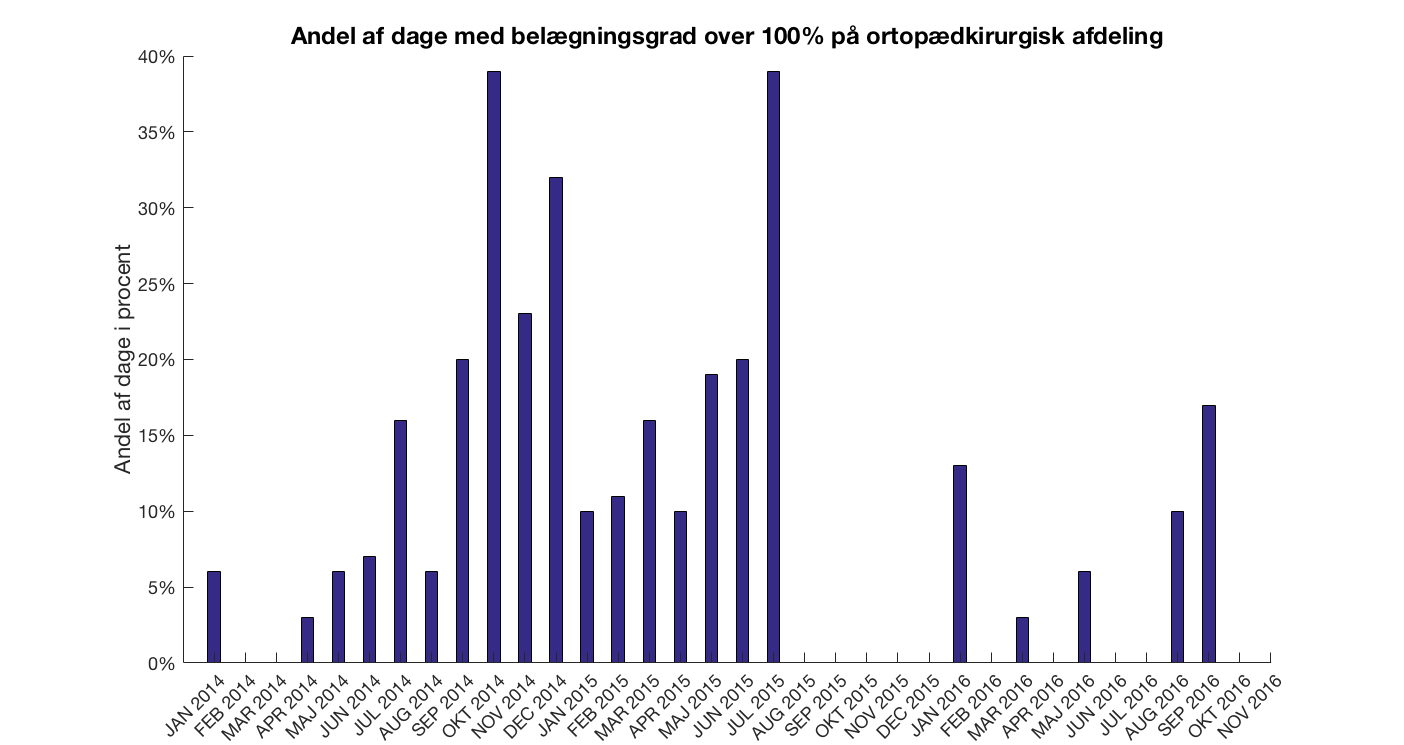
\includegraphics[scale=.7]{figures/antaldage.png}
	\label{antaldage}
	\flushleft
	\caption{\textit{Figuren illustrerer antal dage med en belægningsgrad over $100 \%$ fra januar 			$2014$ til juni $2015$ på ortopædkirugisk afdeling på Aalborg Universitetshospital. 					\cite{SDS2015}}}
\end{figure}


Af \figref{antaldage} ses det, at der i oktober måned år 2014 opleves en belægning på over $100 \%$ i 19 dage. Det vides dog ikke, hvorvidt der er tale om én ekstra eller flere patienter, der udgør en belægningsgrad på over $100 \%$, samt hvor længe patienterne er indlagt på afdelingen. Det ses i \figref{maxminbelaeg}, at der i oktober måned år 2014 opleves en belægning på $130 \%$, hvilket kan opholdes mod de 19 dage. Det skal understreges, at begge grafer er angivet i måneder, og det er derfor uvist om, hvor mange patienter, der er indlagt pr. dag. Derudover er figurerne, \figref{maxminbelaeg} og \figref{antaldage}, udarbejdet over 18 måneder, hvilket angiveligt ikke er en repræsentativ periode for at konkludere et reelt problem på afdelingen. Dertil vides det ikke om belægningsgraden over $100 \%$ opleves som værende et problem på ortopædkirurgisk afdeling på Aalborg Universitetshospital eller om det blot er et strukturerings problem. 